% !TeX root = ../main.tex

\chapter{对Wi-Fi流量的建模}
\label{chap:model}
Wi-Fi流量的变化可以大致分为\emph{短时变化}和\emph{长时变化}两种。短时变化是指短时间内Wi-Fi流量呈现的有无(ON/OFF)变化,通常在毫秒级别,主要是由于Wi-Fi协议中用于媒体访问控制的协议CSMA/CA协议造成的。帧间间隔和退避是产生有无变化的主要原因。长时变化是指Wi-Fi流量在更长时间段内的变化,体现在ON/OFF变化持续时间的分布的变化,通常在小时量级。长时变化在实际生活中有人类活动的变化产生。用户的多少会影响当前环境中Wi-Fi通讯的繁忙与否,从而间接地影响反向散射通讯。本章将对CSMA/CA协议和人类活动带来的影响进行分析,并对信道进行建模。
\section{Wi-Fi流量的有-无状态变化}
\subsection{短时变化:CSMA/CA协议}
IEEE 802.11标准中为解决多个节点同时访问网络所带来的冲突问题,引入了CSMA/CA协议。由于节点是半双工的,不不能同时检测信道状态和发送数据,因此在发送前节点会对当前信道进行监听。CSMA/CA协议中的以下约定使得Wi-Fi流量会出现有-无之间的转变:

\textbf{帧间间隙}(Inter-frame spacing, IFS)。在CSMA/CA中,发一个帧之前,都需要 "等待" 一个相应的帧间间隔,比如发送数据之前至少要等待分布式帧间间隙(DIFS)时间;在收到的数据通过CRC校验后发送ACK之前需要等待短帧间间隔(SIFS)时间。在802.11中还存在其他的一些帧间间隔,比如RIFS,PIFS等。

\textbf{退避}。当基站等待DIFS时间内,信道保持空闲状态,那么会进入退避过程。需要从竞争窗口选择一个随机数。比如默认的初始竞争窗口为31,即随机回退计数值的范围即是$[0,31]$。在退避过程中,每经过一个时隙,节点会监听一次信道,若信道空闲,则相应的随机回退计数器的值减1。递减至0后可以发送数据。若传输中受到干扰,竞争窗口采用二进制指数退避算法扩大竞争窗口,直到成功发送或者窗口大小达到了上限。

这些机制都使得Wi-Fi的数据流呈现ON/OFF之间的不断转换,进而导致利用Wi-Fi信号完成通讯的反向散射方式会在OFF状态下受到影响。
\begin{figure}
	\begin{minipage}[b]{.32\linewidth}
		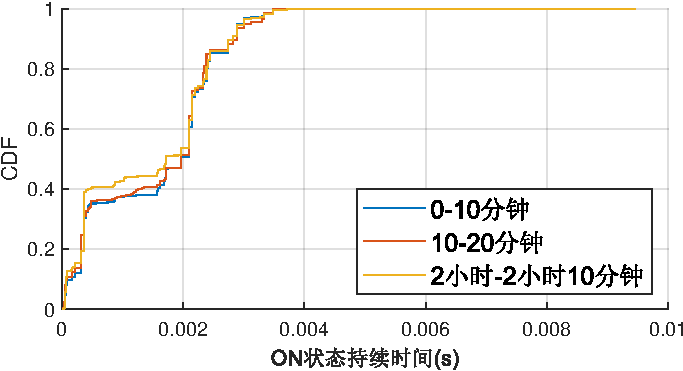
\includegraphics[width = \linewidth]{model_figure1_mall_ON-cropped}
		\subcaption{商场环境,ON状态}\label{fig:ecdf_mall_on}
	\end{minipage}
	\hfill
	\begin{minipage}[b]{.32\linewidth}
		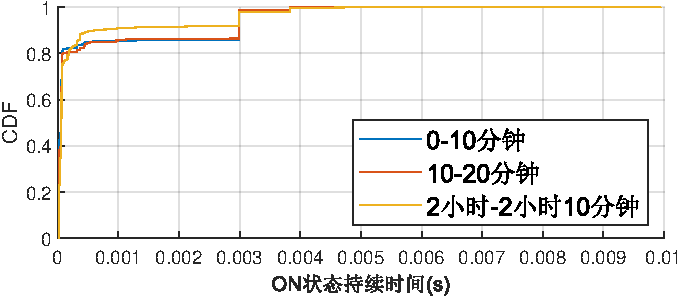
\includegraphics[width = \linewidth]{model_figure1_home_ON-cropped}
		\subcaption{家庭环境,ON状态}\label{fig:ecdf_home_on}
	\end{minipage}
	\hfill
	\begin{minipage}[b]{.32\linewidth}
		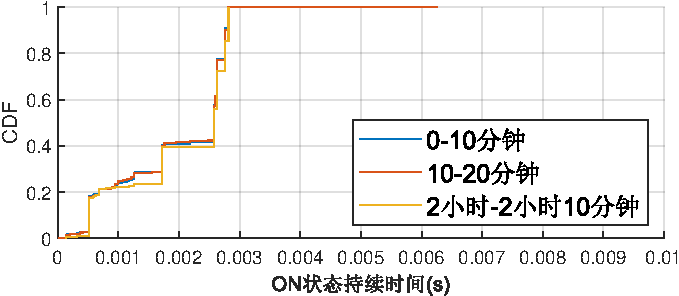
\includegraphics[width = \linewidth]{model_figure1_lab_ON-cropped}
		\subcaption{实验室环境,ON状态}\label{fig:ecdf_lab_on}
	\end{minipage}
	
	\begin{minipage}[b]{.32\linewidth}
		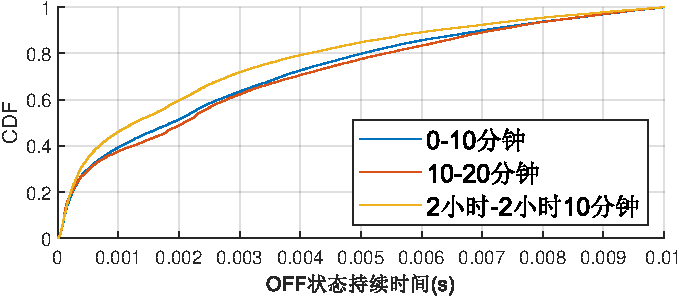
\includegraphics[width = \linewidth]{model_figure1_mall_OFF-cropped}
		\subcaption{商场环境,OFF状态}\label{fig:ecdf_mall_off}
	\end{minipage}
	\hfill
	\begin{minipage}[b]{.32\linewidth}
		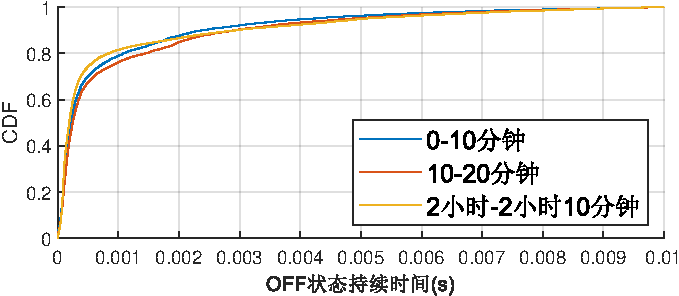
\includegraphics[width = \linewidth]{model_figure1_home_OFF-cropped}
		\subcaption{家庭环境,OFF状态}\label{fig:ecdf_home_off}
	\end{minipage}
	\hfill
	\begin{minipage}[b]{.32\linewidth}
		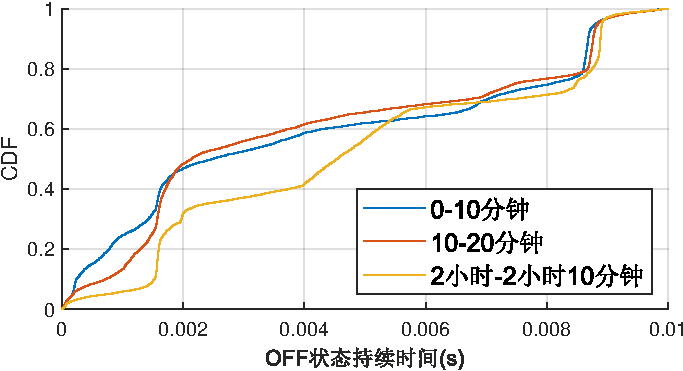
\includegraphics[width = \linewidth]{model_figure1_lab_OFF-cropped}
		\subcaption{实验室环境,OFF状态}\label{fig:ecdf_lab_off}
	\end{minipage}
	\caption{不同环境在不同时间段的Wi-Fi流量ON/OFF状态经验累积分布函数示意图。}\label{fig:ecdf}
\end{figure}
\subsection{长时变化:环境与人类活动}
CSMA/CA协议使得Wi-Fi流量会出现ON/OFF之间的不断转换,但其目的是为了控制共享媒介的使用,而各节点对媒介的使用需求来自环境中用户的需求。因此,当前场景下存在的用户数量以及对网络服务的需求的变化也会使Wi-Fi流量的统计特征产生变化。这种变化有两方面的因素决定:

\textbf{随空间变化}。在不同的环境中Wi-Fi流量的统计分布会有所不同。这主要是由于当前环境的功能不同引起的——环境中用户的数量会影响流量特征。图\ref{fig:ecdf}中展示了商场、家庭、实验室三种不同环境使用USRP采集到的Wi-Fi流量分析。商场中,ON状态持续时间中有两个比较陡峭的上升曲线,且形状比较复杂;OFF状态持续时间分布十分宽广。这大概来源于商场内比较多的用户,因此信道的争抢比较剧烈,导致OFF状态分布广泛。家庭环境中用户比较少,相对的分布更加单纯:ON状态两个陡峭的上升主要来自于长的数据帧的短的控制帧,同时很少的竞争使得两个曲线都比较光滑;在实验室中,ON状态相对商场比较平稳,但比家庭中更复杂,,这是来源于实验室的用户数量介于家庭和商场之间。

\textbf{随时间变化}。图\ref{fig:ecdf}中展示了同一环境下不同时间段的累积分布函数变化。由图可见,相邻的两个时间段(图中红线与蓝线)形状比较相近,而较远的时间段(橙线)会与之前的分布有一定的差异。在家庭中最为稳定,在实验室中最为波动。
\section{统计建模}
\label{sec:model}
在了解CSMA/CA协议的基础上,最直观的方式便是对当前环境下的Wi-Fi信道进行\emph{仿真模拟}。在给定当前场景下的节点数目、每个节点的数据传输模式,便可以遵循CSMA/CA协议对ON/OFF状态进行模拟。但是进行这样模拟存在如下的问题:

\textbf{参数的确定}。确定环境中接入节点的数量并非在所有的情境下都可以实现;即便可以确定,对于每个节点的传输模式也需要确定如何进行数据的传输模式。另一方面,考虑到Wi-Fi流量随时间的变化,模拟的参数也要是随时变的。这会使得需要确定的参数比较复杂。

\textbf{计算的复杂度}。由于各个节点之间是相互影响的,因此在计算的时候需要为每一个节点维护当前发送的状态;同时在计算每一时刻的有-无状态时,需要考虑所有的节点。最后,为了获得统计上的稳定值,需要进行多次模拟去期望。这都使得直接对当前环境中存在的节点进行模拟有较高的复杂度。

%加上关于Hurst的部分
考虑到以上几点,一个更加合适的方案是\emph{直接对环境中Wi-Fi信号的ON/OFF变化进行统计模拟},而非考虑各个节点的传输状态。Wi-Fi信号的一个特征是有较强的\emph{持续性}——如果当前处于ON状态,会有很高的可能性留在ON状态;对于OFF庄涛也是同理。这一特征已经在许多文献\cite{}中得到讨论。具体来讲,Wi-Fi流量具有比较高的赫斯特指数(Hurst exponent),而赫斯特指数用来描述一个时间序列的长程记忆性,越高的赫斯特指数表明时间序列有越强的可预测性。对Wi-Fi流量构成的时间序列来讲,其赫斯特指数在0.75-0.90的范围内,可以被认定为有较强的持续性。

这一特性提供了使得统计ON/OFF状态持续时间的理论基础。由于环境中Wi-Fi信号在ON/OFF两种状态之间不断转换,那么对ON状态下的Wi-Fi信号持续长度和OFF状态下的Wi-Fi信号持续长度进行统计,再按照相应的分布函数即可实现对
对由CSMA/CA协议造成的ON/OFF状态变化,我们使用马尔科夫链进行模拟,对每个状态又用经验的累积分布函数进行描述;而由人类活动变化造成的长时变化,我们利用滑动窗口实现时变的特性。

\textbf{受马尔科夫链控制的信道}。
Wi-Fi在ON/OFF两个状态之间的交替变化
可以用这样的两序列描述:
\begin{equation}
\label{equ:state}
(s_1, \,  s_2, \, s_3 , \, s_4, \cdots),
\end{equation}
\begin{equation}
\label{equ:time}
(t_{1}, \, t_{2}, \, t_{3}, \, t_{4}, \cdots),
\end{equation}
其中,随机变量$S$定义在状态空间$\Omega_1 = \{ON,OFF\}$上,表示当前环境中Wi-Fi信号的有无;随机变量$T$定义在状态空间$\Omega_2 = \{t > 0 | t \in \mathbb{R}\}$上,表示对应状态的持续时间。

在实际状态中,“ON/OFF两种状态的变化是交替的,可以用一个固定转变状态的马尔科夫链描述。
同时,式\ref{equ:state}可以省略。因此,这种描述进一步简化为
由一串\emph{ON/OFF状态持续的时间长度序列}。如果定义随机变量$T_{ON}$为ON状态下的持续时长,定义随机变量$T_{OFF}$为OFF状态下的持续时长,那么
在$S = ON$的状态下,$T = T_{ON}$,服从由历史Wi-Fi流量中有状态持续时间统计的累积分布函数$F_{ON}$;在$S = OFF$的状态下,$T = T_{OFF}$,服从经验累积分布函数$F_{OFF}$。状态持续时间受马尔科夫链控制。

状态$S$不仅决定了当前随机变量$T$的具体分布,还决定了当前信道的特性。在$S = ON$的状态下,信道可以简单的模拟为加性高斯信道;在$S = OFF$的状态下,信道是一个“归零”加性高斯信道——不论信源传输的是1或是0,都会被归0\footnote{这是在采用OOK的情况下,比特1被调制为幅度为$a$的信号,比特0被调制为幅度为0的信号。},然后经过一个普通的加性高斯信道。同样,当前信道
也受马尔科夫链控制。

图\ref{fig:markov_model}为模型的图示。ON/OFF两种状态以$1$的确定概率相互转换,不同状态下$T$服从不同的分布,此时信道的状态也相应地在普通加性高斯信道和“归零”信道之间变化。

\textbf{滑动窗口}。由于实际场景中,人类活动的变化会造成Wi-Fi流量的变化,因此我们需要引入时间上的变化以及时地更新统计信息$F_{ON},F_{OFF}$。在实现中,我们会记录上一时间区间内,帧的长度以及帧间间隔的信息,依据这些信息更新$F_{ON},F_{OFF}$,用于下一时段内的预测和优化。
\begin{figure}[t]
	\begin{minipage}[b]{.5\linewidth}
		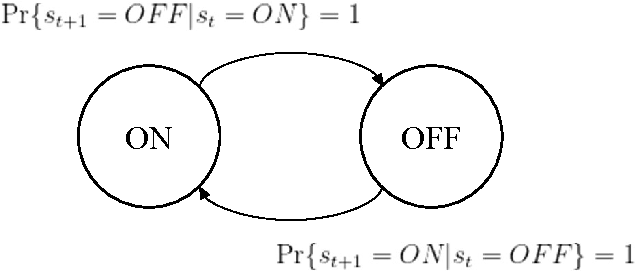
\includegraphics[width = \linewidth]{model_figure4_markov-cropped}
		\subcaption{马尔可夫链。ON/OFF两状态相互转换。}\label{fig:markov_chain}
	\end{minipage}
	\hfill
	\begin{minipage}[b]{.5\linewidth}
		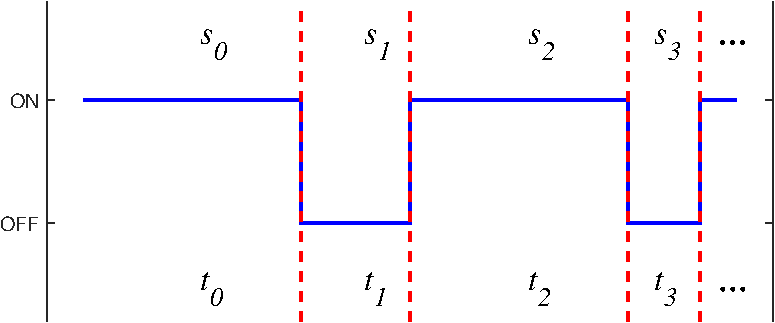
\includegraphics[width = \linewidth]{model_figure4_onOFF-cropped}
		\subcaption{由两序列描述的Wi-Fi流量状态变化。}\label{fig:series}
	\end{minipage}
	\caption{受马尔可夫链控制的信道模型。}\label{fig:markov_model}
\end{figure}